\documentclass{article}
\usepackage[utf8]{inputenc}
\usepackage{pgfplots}
\pgfplotsset{compat=1.17}
\usepackage{graphicx}

\title{Math 215 Homework 4 Question 7}

\begin{document}

\section{Math 215 Homework 4 Question 7}


Reduce to Standard Form and State the shape \\ \\
24: $y^2 = x^2 + 4z^2 + 4$\\ 
$ y^2 - x^2 - 4z^2 = 4$ \\
$ \frac{y^2}{4} - \frac{x^2}{4} - z^2 = 1$ \\ \\
shape is a hyperboliod of two sheets 
\\
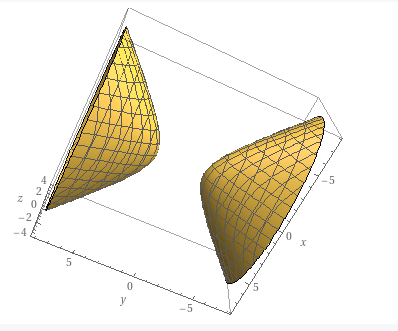
\includegraphics{hyperbaloid of two sheets.png}

\pagebreak
25: $4x^2 + y^2 +4z^2 -4y-24z+36 = 0$ \\
$4x^2 +y^2 +4(z^2-6z+9) = 0$ \\
$4x^2 + y^2 - 4y +4(z-3)^2 = 0$\\
$4x^2+y^2-4y+4 +4(z-3)^2 =4$ \\
$4x^2+(y-2)^2 +4(z-3)^2 =4$ \\
$x^2+\frac{(y-2)^2}{4} +(z-3)^2 =1$ \\ \\
shape is an ellipsoid
\\
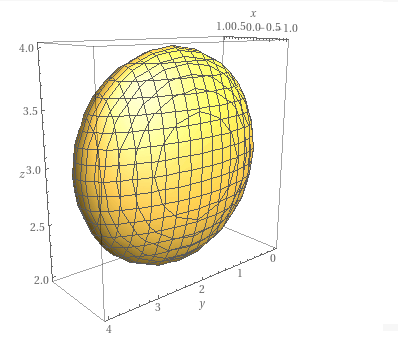
\includegraphics{ellipsoid.png}
\\ \\ \\
26: $4y^2 + z^2 -x - 16y -4z + 20 = 0$\\
$4y^2 -16y +16 + z^2  -4z + 4 = x$\\
$4(y^2 -4y +4) + z^2  -4z + 4 = x$\\
$4(y-2)^2 + (z-2)^2 = x$\\
$(y-2)^2 + \frac{(z-2)^2}{4} = \frac{x}{4}$\\ \\
shape is an elliptic parabaloid



\end{document}